One approach to calculating the area of quadrilateral $PUTS$ is to divide it into triangle $PQU$, triangle $SRT$, and trapezoid $QUTR$. A trapezoid is a quadrilateral with only one pair of parallel sides. To compute these areas, we need the heights $h_1$ and $h_2$. To calculate $h_1$, apply the Pythagoras theorem to triangle $OQU$. And likewise $h_2$ with triangle $ORT$. 
\begin{figure}[H]
\centering
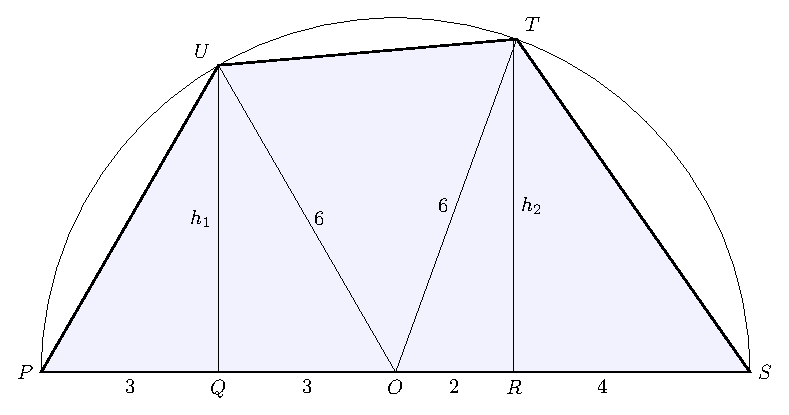
\includegraphics[height=5cm]{quadrilateral-inscribed-labeled}
\end{figure}
\begin{align*}
h_1 & = \sqrt{6^2 -3^2} = \sqrt{27} = 3\sqrt{3} \approx 5.196 \\
h_2 & = \sqrt{6^2 -2^2} =\sqrt{32} = 4\sqrt{2} \approx 5.657
\end{align*}
The area of triangle $PQU$ and $SRT$ are:
\begin{align*}
\frac{1}{2} \times 3 \times h_1 & = 4.5\sqrt{3} \approx 7.794 \\
\frac{1}{2} \times 4 \times h_2 & = 8\sqrt{2} \approx 11.314 
\end{align*}
The area of trapezoid $QUTR$ equals the area of a parallelogram with equal base and height equal to the average height. 
\begin{align*}
QR \times \frac{h_1+h_2}{2} 
  = 5 \times \frac{3\sqrt{3}+4\sqrt{2}}{2}
  = 10\sqrt{2} + 7.5\sqrt{3}
  \approx 27.133 
\end{align*}
Adding up the areas of the triangles and trapezoid yields:
\begin{align*}
4.5\sqrt{3} + 8\sqrt{2} + 7.5\sqrt{3} + 10\sqrt{2}
  = 18\sqrt{2} + 12\sqrt{3}
  \approx 46.240
\end{align*}
\begin{empheq}[box={\mathbox[colback=white]}]{equation*}
    46.2~\text{units}^2
\end{empheq}
